\documentclass[11pt,letterpaper]{article}
\usepackage[T1]{fontenc}
\usepackage[scaled]{helvet}
\renewcommand{\familydefault}{\sfdefault}
\usepackage{amsmath,amssymb}
\usepackage[margin=0.8in,bottom=0.9in]{geometry}
\usepackage[most]{tcolorbox}
\usepackage{tikz}
\usetikzlibrary{calc}
\usepackage{enumitem}
\usepackage{array}
\usepackage{needspace}
\usepackage{fancyhdr}
\usepackage{pifont}

% ---- Palette "F. Bright & Playful" ----
\definecolor{fmtitle}{HTML}{3D2C8D}
\definecolor{fmkey}{HTML}{0096C7}
\definecolor{fmwatch}{HTML}{2BB673}
\definecolor{fmturn}{HTML}{F4A100}
\definecolor{fmmistake}{HTML}{EF476F}
\definecolor{fmnotice}{HTML}{9B5DE5}
\definecolor{fmgray}{HTML}{6B6B6B}

\pagestyle{fancy}
\fancyhf{}
\renewcommand{\headrulewidth}{0pt}
\fancyfoot[C]{\footnotesize\color{fmgray}\textcopyright\ 2026 FangMath. All rights reserved.}
\fancyfoot[R]{\footnotesize\color{fmgray}\thepage}
\setlength{\parindent}{0pt}
\setlength{\parskip}{3pt}

\newcommand{\badge}[1]{\colorbox{fmtitle}{\color{white}\bfseries\small\ #1\ }}
\newcommand{\leveltag}[2]{\colorbox{#1}{\color{white}\bfseries\scriptsize\ #2\ }}
\newcommand{\LE}{\leveltag{fmwatch}{EASY}}
\newcommand{\LM}{\leveltag{fmturn}{MEDIUM}}
\newcommand{\LH}{\leveltag{fmmistake}{HARD}}

\newcommand{\sectionbar}[2]{\needspace{6cm}\par\vspace{4mm}
  \begin{tcolorbox}[enhanced,colback=fmtitle,colframe=fmtitle,arc=2mm,
    left=4mm,top=1.5mm,bottom=1.5mm]
  \color{white}\bfseries\large #1\hfill{\normalsize\mdseries #2}
  \end{tcolorbox}}

\newtcolorbox{keyidea}{enhanced,breakable,colback=white,colframe=fmkey,boxrule=1pt,arc=2mm,
  title={Key Idea},coltitle=fmkey,fonttitle=\bfseries,
  attach boxed title to top left={xshift=4mm,yshift=-2mm},
  boxed title style={colback=white,colframe=fmkey,boxrule=0.9pt}}
\newtcolorbox{watchme}{enhanced,colback=white,colframe=fmwatch,boxrule=1pt,arc=2mm,
  title={Watch Me --- Worked Example},coltitle=fmwatch,fonttitle=\bfseries,
  attach boxed title to top left={xshift=4mm,yshift=-2mm},
  boxed title style={colback=white,colframe=fmwatch,boxrule=0.9pt}}
\newtcolorbox{mistakebox}{enhanced,breakable,colback=white,colframe=fmmistake,boxrule=1pt,arc=2mm,
  title={Common Mistake},coltitle=fmmistake,fonttitle=\bfseries,
  attach boxed title to top left={xshift=4mm,yshift=-2mm},
  boxed title style={colback=white,colframe=fmmistake,boxrule=0.9pt}}
\newtcolorbox{yourturn}{enhanced,breakable,colback=white,colframe=fmturn,boxrule=1pt,arc=2mm,
  title={Your Turn},coltitle=fmturn,fonttitle=\bfseries,
  attach boxed title to top left={xshift=4mm,yshift=-2mm},
  boxed title style={colback=white,colframe=fmturn,boxrule=0.9pt}}
\newtcolorbox{answerbox}[1]{enhanced,breakable,colback=white,colframe=fmwatch,boxrule=1pt,arc=2mm,
  title={#1},coltitle=fmwatch,fonttitle=\bfseries,
  attach boxed title to top left={xshift=4mm,yshift=-2mm},
  boxed title style={colback=white,colframe=fmwatch,boxrule=0.9pt}}

\newcommand{\work}[1]{\par\vspace{#1}}
\setlist[enumerate]{itemsep=2pt,topsep=3pt}

% ---------------- extra boxes ----------------
\newtcolorbox{notebox}{enhanced,breakable,colback=white,colframe=fmnotice,boxrule=1pt,arc=2mm,
  title={Notice},coltitle=fmnotice,fonttitle=\bfseries,
  attach boxed title to top left={xshift=4mm,yshift=-2mm},
  boxed title style={colback=white,colframe=fmnotice,boxrule=0.9pt}}
\newtcolorbox{exbox}{enhanced,colback=white,colframe=fmwatch,boxrule=0.8pt,arc=2mm,
  title={Example},coltitle=fmwatch,fonttitle=\bfseries\small,
  attach boxed title to top left={xshift=4mm,yshift=-2mm},
  boxed title style={colback=white,colframe=fmwatch,boxrule=0.8pt},fontupper=\small}
\newcommand{\topicbar}[1]{\needspace{4.5cm}\par\vspace{5mm}
  \begin{tcolorbox}[enhanced,colback=fmtitle,colframe=fmtitle,arc=2mm,left=4mm,top=1.5mm,bottom=1.5mm]
  \color{white}\bfseries\large #1
  \end{tcolorbox}}
\usepackage{multicol}

% ---------------- practice layout ----------------
\newcommand{\workline}{\par\vspace{7mm}{\color{gray!55}\rule{\linewidth}{0.4pt}}}
\newcommand{\worklines}[1]{\foreach \i in {1,...,#1}{\workline}}
\newcommand{\prob}[3]{\needspace{#3}\par\vspace{3mm}{\color{fmturn}\bfseries #1.}\ #2\par}
\newcommand{\ansline}{\par\vspace{4mm}\hfill\textbf{Answer:}\ \rule{5cm}{0.4pt}\par}
\newcommand{\keyitem}[3]{\needspace{3.2cm}\par\vspace{2mm}
  \begin{tcolorbox}[enhanced,colback=white,colframe=fmwatch!60,boxrule=0.6pt,arc=1.5mm,left=3mm,top=1.5mm,bottom=1.5mm]
  {\color{fmwatch}\bfseries #1.}\quad\small #2\par\vspace{1mm}
  \normalsize\textbf{Answer: #3}
  \end{tcolorbox}}


\usetikzlibrary{arrows.meta}
\providecommand{\iskey}{0}
% fill-in blank: line for students, pink answer in the key
\newcommand{\fb}[2][2.6cm]{\ifnum\iskey=1 \underline{\makebox[#1][c]{\color{fmmistake}\bfseries #2}}\else\underline{\makebox[#1]{}}\fi}
% answer line for practice problems
\newcommand{\pans}[2][3.2cm]{\ifnum\iskey=1 \underline{\makebox[#1][c]{\color{fmmistake}\bfseries #2}}\else\rule{#1}{0.4pt}\fi}
\newcommand{\vid}[1]{{\color{fmgray}\small\textit{\ding{43} Video: #1}}}
\newcommand{\pt}[2]{\fill (#1) circle (2.2pt) node[above=1pt,font=\small]{$#2$};}

\usetikzlibrary{decorations.pathreplacing}
% three points on a segment with lengths written above the pieces: #1,#2,#3 letters; #4,#5 piece labels; #6 whole label (below)
\newcommand{\threept}[6]{\begin{tikzpicture}[x=1cm]\draw[thick] (0,0)--(3.6,0);
\fill (0,0) circle(2.2pt) node[below=2pt,font=\small]{$#1$} (1.4,0) circle(2.2pt) node[below=2pt,font=\small]{$#2$} (3.6,0) circle(2.2pt) node[below=2pt,font=\small]{$#3$};
\node[above,font=\small] at (0.7,0.02){#4};\node[above,font=\small] at (2.5,0.02){#5};
\if\relax\detokenize{#6}\relax\else\draw[gray,decorate,decoration={brace,amplitude=4pt,mirror}] (0,-0.45)--(3.6,-0.45) node[midway,below=4pt,font=\small]{#6};\fi
\end{tikzpicture}}
\newcommand{\sdp}[3]{\begin{minipage}[t][2.4cm]{0.48\linewidth}{\color{fmturn}\bfseries #1.}\ #2\par\vfill\hfill \pans[3.6cm]{#3}\end{minipage}}
\newcommand{\figp}[4]{\begin{minipage}[t]{0.48\linewidth}{\color{fmturn}\bfseries #1.}\ #2\par\vspace{1mm}\centering #3\par\vspace{2mm}\raggedleft \pans[2.6cm]{#4}\end{minipage}}
\newcommand{\algp}[3]{\begin{minipage}[t][4.6cm]{0.48\linewidth}{\color{fmturn}\bfseries #1.}\ #2\par\vfill\hfill \pans[4.2cm]{#3}\end{minipage}}


% ch2: long key answers wrap inside their column instead of running into the next one
\newlength{\pw}
\renewcommand{\pans}[2][3.2cm]{\ifnum\iskey=1 \settowidth{\pw}{\bfseries #2}\ifdim\pw>#1 \parbox[b]{#1}{\raggedleft\color{fmmistake}\bfseries\small #2}\else\underline{\makebox[#1][c]{\color{fmmistake}\bfseries #2}}\fi\else\rule{#1}{0.4pt}\fi}
% parallel lines l, m cut by transversal t; #1 = comma list of angle numbers to highlight
\newcommand{\tfig}[1][]{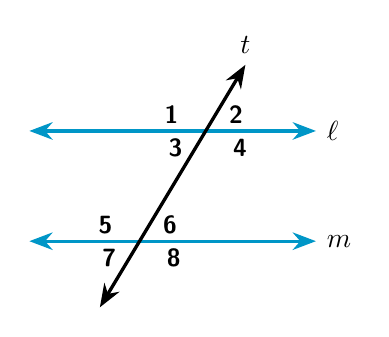
\begin{tikzpicture}[scale=0.7]
\draw[very thick,fmkey,{Stealth}-{Stealth}] (-2.6,1)--(2.6,1) node[right,black]{$\ell$};
\draw[very thick,fmkey,{Stealth}-{Stealth}] (-2.6,-1)--(2.6,-1) node[right,black]{$m$};
\draw[very thick,{Stealth}-{Stealth}] (-1.32,-2.2)--(1.32,2.2) node[above]{$t$};
\foreach \n/\x/\y in {1/-0.02/1.3,2/1.15/1.3,3/0.05/0.7,4/1.22/0.7,5/-1.22/-0.7,6/-0.05/-0.7,7/-1.15/-1.3,8/0.02/-1.3}{\node[font=\small\bfseries] at (\x,\y){\n};}
\end{tikzpicture}}
\begin{document}
\ifnum\iskey=1 \colorbox{fmwatch}{\color{white}\bfseries\small\ ANSWER KEY\ }\else\badge{PRACTICE}\fi\hfill{\small\color{fmgray}Geometry \textperiodcentered\ Lesson 3.4}\par\vspace{4mm}
{\color{fmtitle}\LARGE\bfseries Perpendicular Lines --- Practice\ifnum\iskey=1 \ --- Answer Key\fi}\par\vspace{1mm}
{\color{fmgray}A worked example comes before each type. Show your thinking.}\par\vspace{3mm}
Name: \rule{6cm}{0.4pt}\hspace{1cm}Date: \rule{3.5cm}{0.4pt}\par\vspace{2mm}


\needspace{6cm}\topicbar{Type 1 \quad Right Angles and Perpendicular Lines}
\begin{watchme}$\overleftrightarrow{AB} \perp \overleftrightarrow{CD}$ at $E$, and $m\angle AEF = 35^\circ$ with $\overrightarrow{EF}$ between $\overrightarrow{EA}$ and $\overrightarrow{EC}$.\par
$\angle AEC = 90^\circ$, so $m\angle FEC = 90 - 35 = 55^\circ$. \quad \textbf{Answer: $\boldsymbol{55^\circ}$}\end{watchme}
\needspace{3.4cm}\noindent\sdp{1}{$a \perp b$. What is the measure of each of the four angles they form?}{$90^\circ$}\hfill\sdp{2}{Two lines form a linear pair of congruent angles. What can you conclude?}{the lines are perpendicular}\par\vspace{2mm}
\needspace{4.6cm}\noindent\algp{3}{Two lines are perpendicular. One angle is $(3x + 15)^\circ$. Find $x$.}{$x = 25$}\hfill\algp{4}{$\overrightarrow{BD}$ is inside right angle $\angle ABC$. $m\angle ABD = (2x)^\circ$, $m\angle DBC = (x + 18)^\circ$. Find $x$.}{$x = 24$}\par

\needspace{6cm}\topicbar{Type 2 \quad Perpendicular to the Same Line}
\begin{watchme}In a plane, $p \perp t$ and $q \perp t$. \ Both make $90^\circ$ corresponding angles with $t$, so $p \parallel q$.\end{watchme}
\needspace{3.4cm}\noindent\sdp{5}{In a plane, $a \perp c$ and $b \perp c$. How are $a$ and $b$ related?}{$a \parallel b$}\hfill\sdp{6}{$a \parallel b$ and $c \perp a$. How are $c$ and $b$ related?}{$c \perp b$}\par

\needspace{6cm}\topicbar{Type 3 \quad Distance From a Point to a Line}
\begin{watchme}\begin{minipage}[c]{0.3\linewidth}\centering 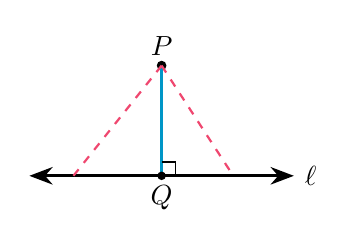
\begin{tikzpicture}[scale=0.7]\draw[very thick,{Stealth}-{Stealth}] (-2.4,0)--(2.4,0) node[right]{$\ell$};\fill (0,2) circle(2.5pt) node[above]{$P$};\draw[very thick,fmkey] (0,2)--(0,0);\fill (0,0) circle(2.2pt) node[below]{$Q$};\draw (0,0)--(0.25,0)--(0.25,0.25)--(0,0.25);\draw[thick,dashed,fmmistake] (0,2)--(-1.6,0) (0,2)--(1.3,0);\end{tikzpicture}\end{minipage}\hfill
\begin{minipage}[c]{0.66\linewidth}Point $(-2, 7)$ and the line $y = 3$. \ Straight down to $(-2, 3)$: distance $= 7 - 3 = 4$.\par
Point $(5, 1)$ and the line $x = -1$. \ Straight across to $(-1, 1)$: distance $= 5 - (-1) = 6$.\end{minipage}\end{watchme}
\needspace{3.4cm}\noindent\sdp{7}{Distance from $(4, 9)$ to the line $y = 2$.}{$7$}\hfill\sdp{8}{Distance from $(-3, -1)$ to the line $y = 4$.}{$5$}\par\vspace{2mm}
\needspace{3.4cm}\noindent\sdp{9}{Distance from $(6, 2)$ to the line $x = 1$.}{$5$}\hfill\sdp{10}{Distance from $(-4, 0)$ to the $y$-axis.}{$4$}\par\vspace{2mm}
\needspace{3.4cm}\noindent\sdp{11}{From $P$, the segments to line $\ell$ have lengths $9$, $6$, $7.5$ and $11$. Which could be the distance from $P$ to $\ell$?}{$6$ (the shortest)}\hfill\sdp{12}{\LH\ The parallel lines $y = 2x + 1$ and $y = 2x + 6$ are $5$ apart measured straight up. Is the distance between them $5$? Why?}{no --- a vertical segment is not perpendicular to them, so the distance is less than 5}\par
\end{document}
